\section{Hardware Implementation Results}

\subsection{Simulation}

\subsubsection{Testbench}

\lstinputlisting[style=StyleCode ,language=SystemVerilog, caption={Testbench for Waveform Generator.}]{./../03_verif/wave_gen_tb.sv}

\subsubsection{Results of Wave Simulation}
\begin{figure}[H]
	\centering
	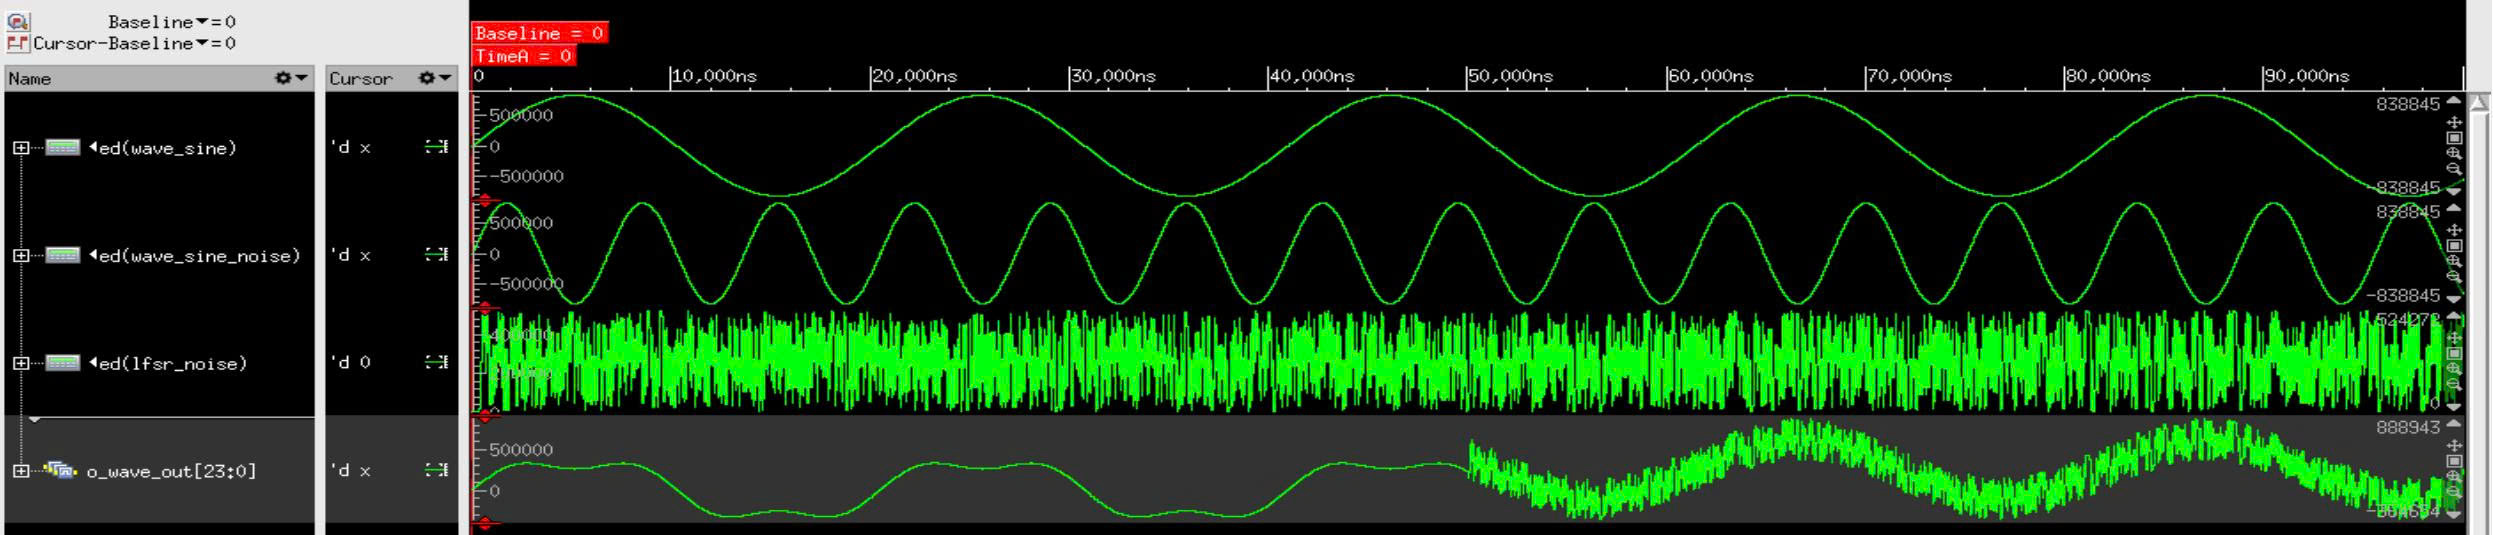
\includegraphics[width=.9\linewidth]{./my-chapters/my-images/simulation/sin_add_noise_sin.jpg}
	\caption{A sine wave affected by third-order harmonic sine noise and white noise.}
\end{figure}

\begin{figure}[H]
	\centering
	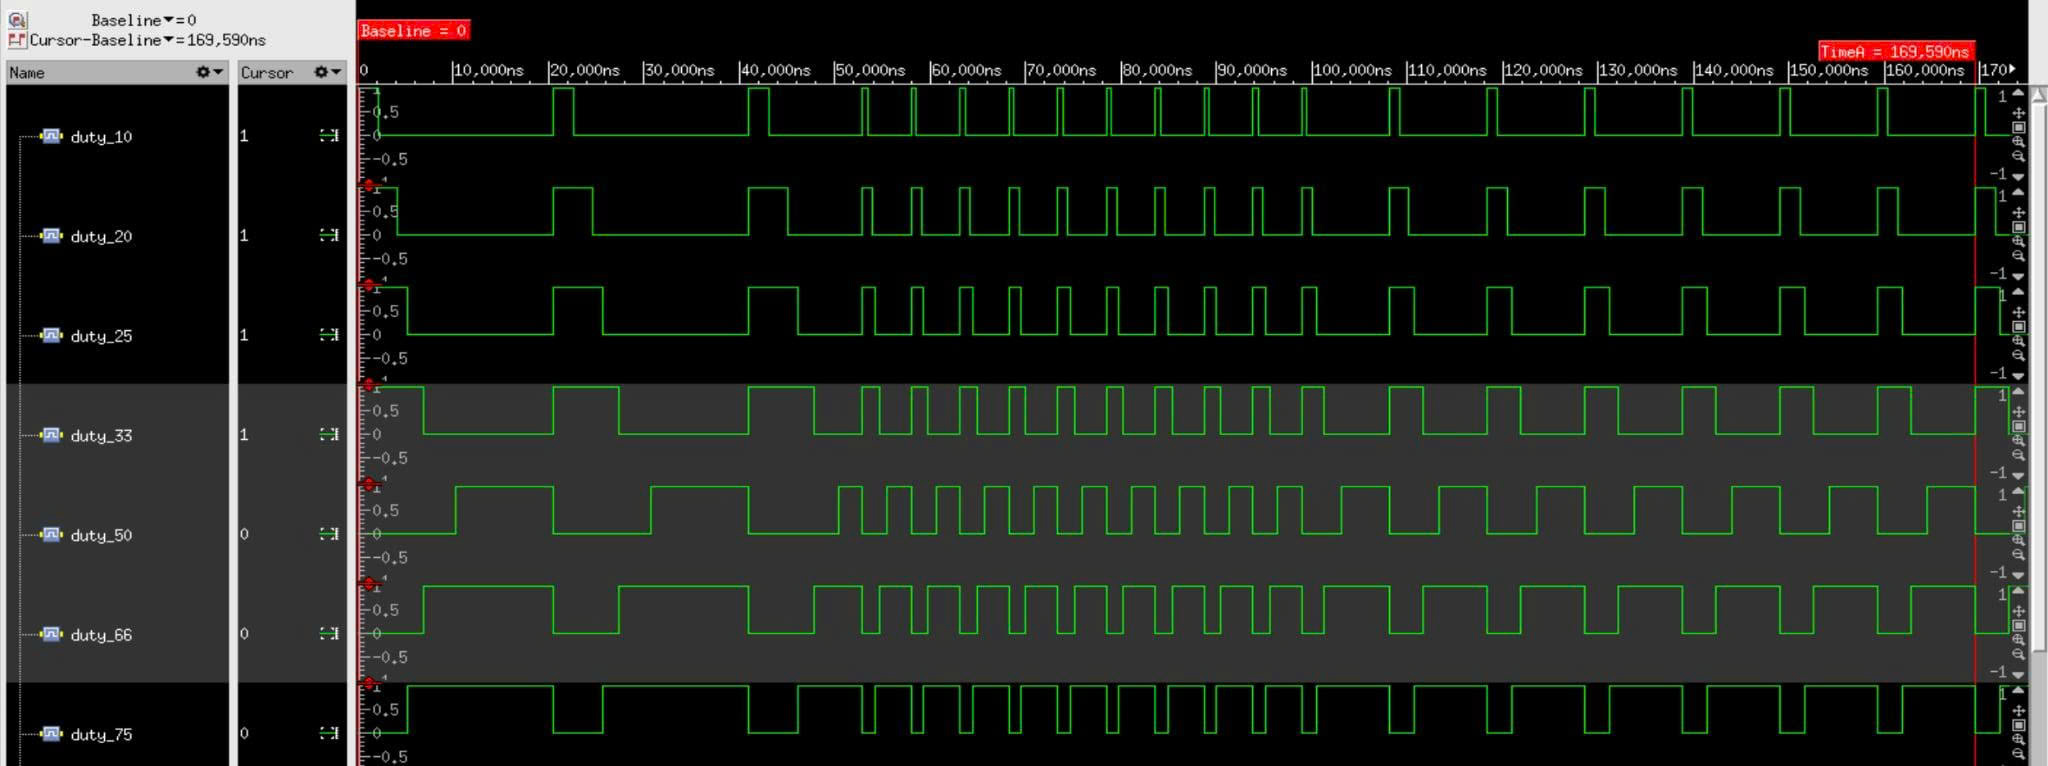
\includegraphics[width=.9\linewidth]{./my-chapters/my-images/simulation/duty_cycle.jpg}
	\caption{Demonstration of square waves with different duty cycles ranging from 10\% to 90\%.}
\end{figure}

\begin{figure}[H]
	\centering
	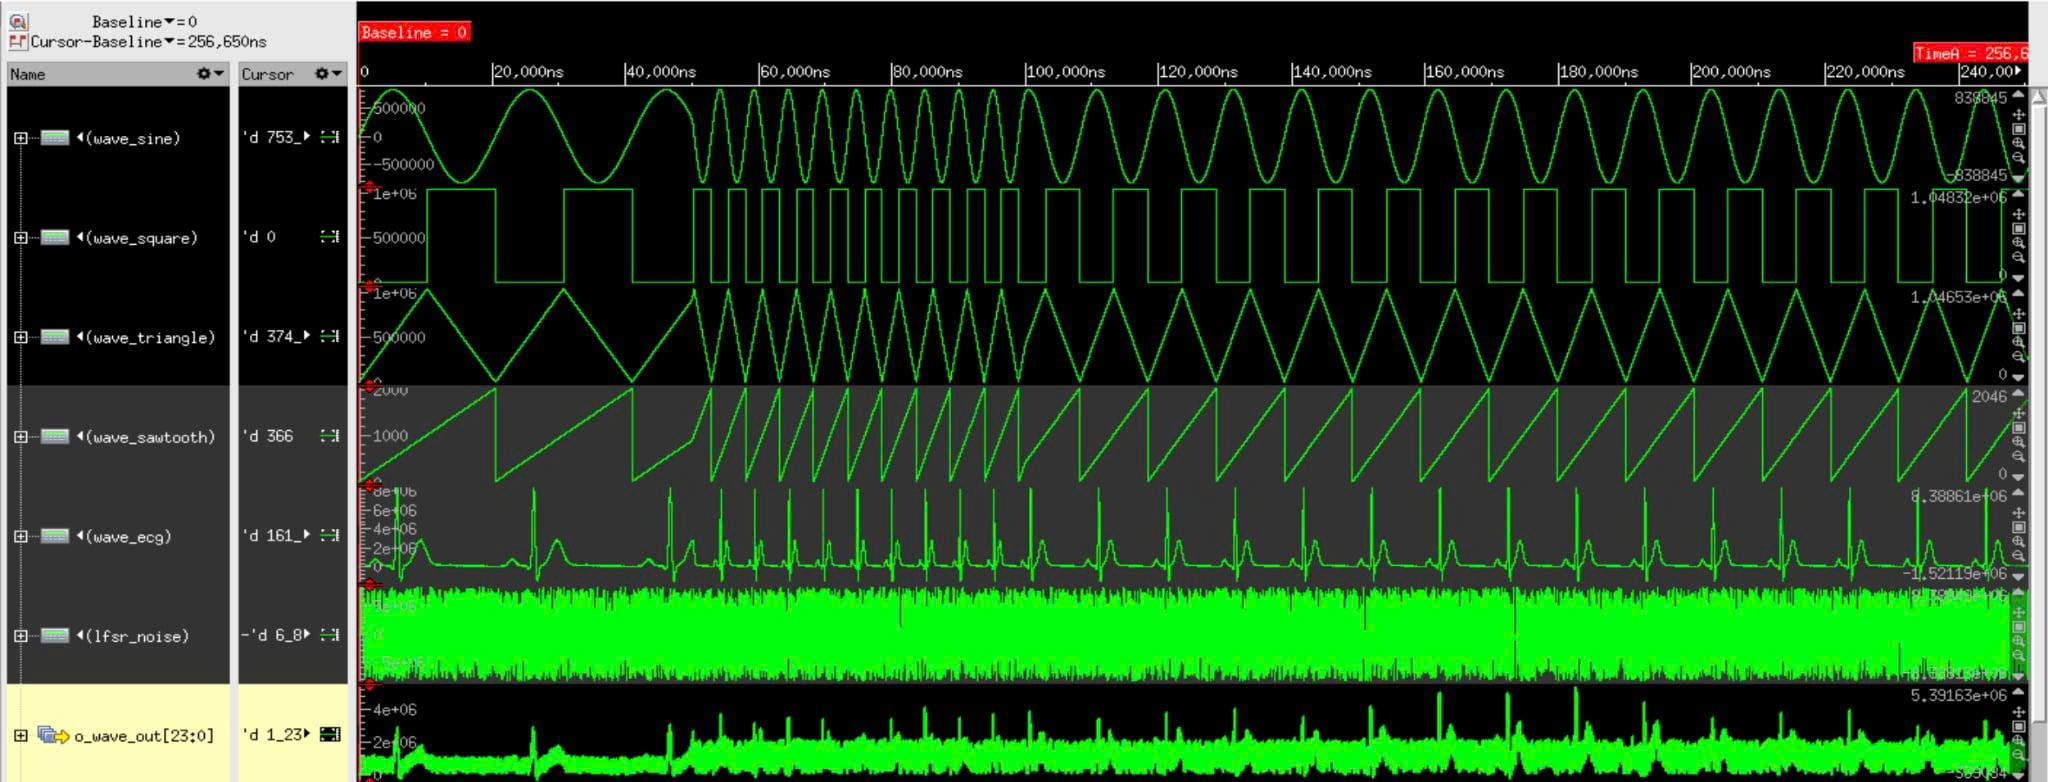
\includegraphics[width=.9\linewidth]{./my-chapters/my-images/simulation/waveform_with_noise.jpg}
	\caption{Basic waveforms and noise modulation: ECG output signal affected by frequency and amplitude variations of injected noise.}
\end{figure}

\begin{table}[H]
	\centering
	\begin{tabular}{|c|m{3cm}|m{10cm}|c|}
		\hline
		\textbf{No.} & \textbf{Testcase} & \textbf{Description} & \textbf{Result} \\
		\hline
		1 & RESET & System reset, the output always zero & PASS \\
		\hline
		2 & Wave generation & Generation success of 5 types of wave: sine, square, triangle, sawtooth and ECG. 
		These waves can adjust frequency and amplitude at the output. 
		In the case of the square wave, it provides the ability to adjust duty cycle from 10\% to 90\%. & PASS \\
		\hline
		3 & Noise generation & Successful generation of white noise (using LFSR for modeling white noise) and one high-frequency sine wave (harmonic of sine wave). 
		These waves can adjust frequency and amplitude at the output. & PASS \\
		\hline
		4 & Wave add noise & The system output can optionally add noise to the main wave, with selectable white noise or harmonic of sine wave. & PASS \\
		\hline
	\end{tabular}
	\caption{Testcase results}
\end{table}

\subsection{Top module}

\begin{figure}[H]
	\centering
	\fbox{%
		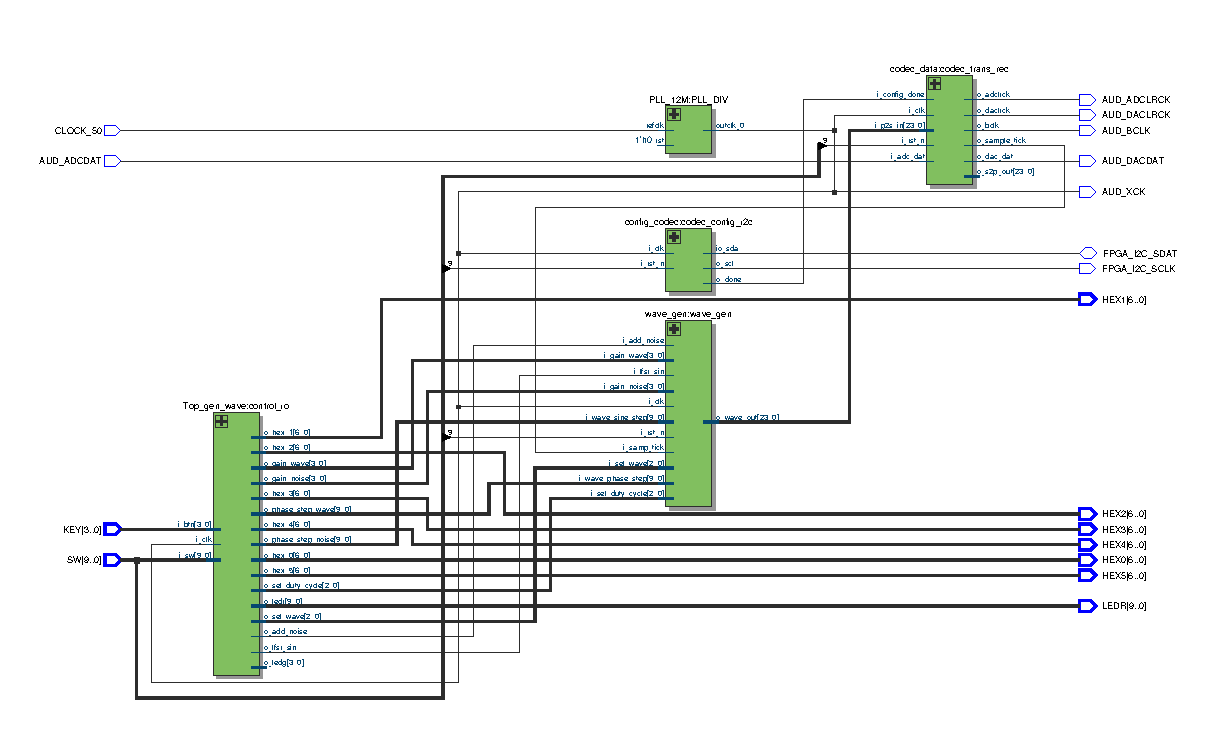
\includegraphics[width=\linewidth]{./my-chapters/my-diagrams/top_image.pdf}%
	}
	\caption{Block diagram for Top module.}
\end{figure}

\subsection{Measurement Waveform}

\begin{figure}[H]
	\centering
	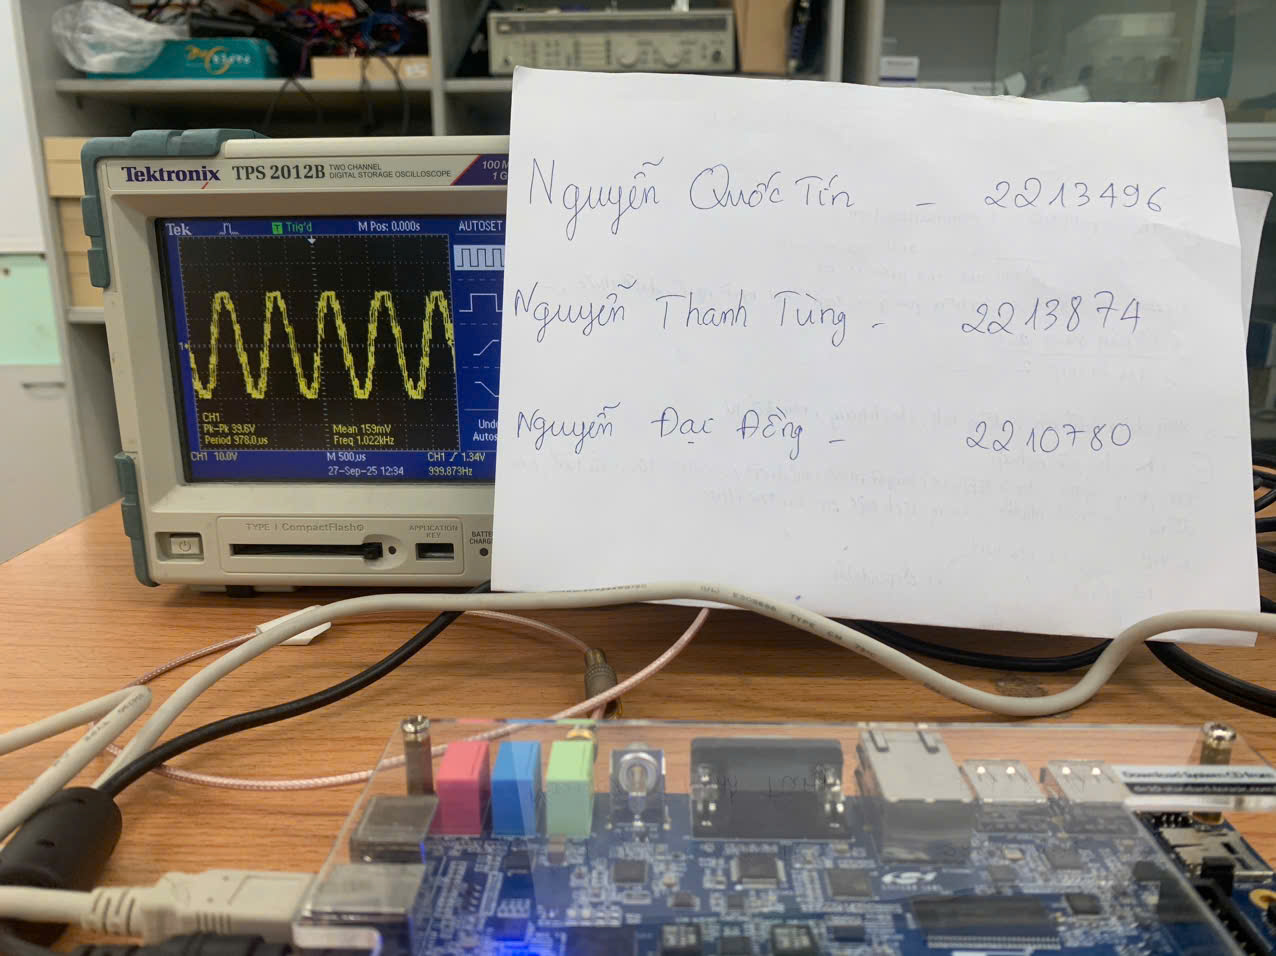
\includegraphics[width=.9\linewidth]{./my-chapters/my-images/Gen_wave/hinh2.jpg}
	\caption{Sine waveform on Oscilloscope.}
\end{figure}

\begin{figure}[H]
	\centering
	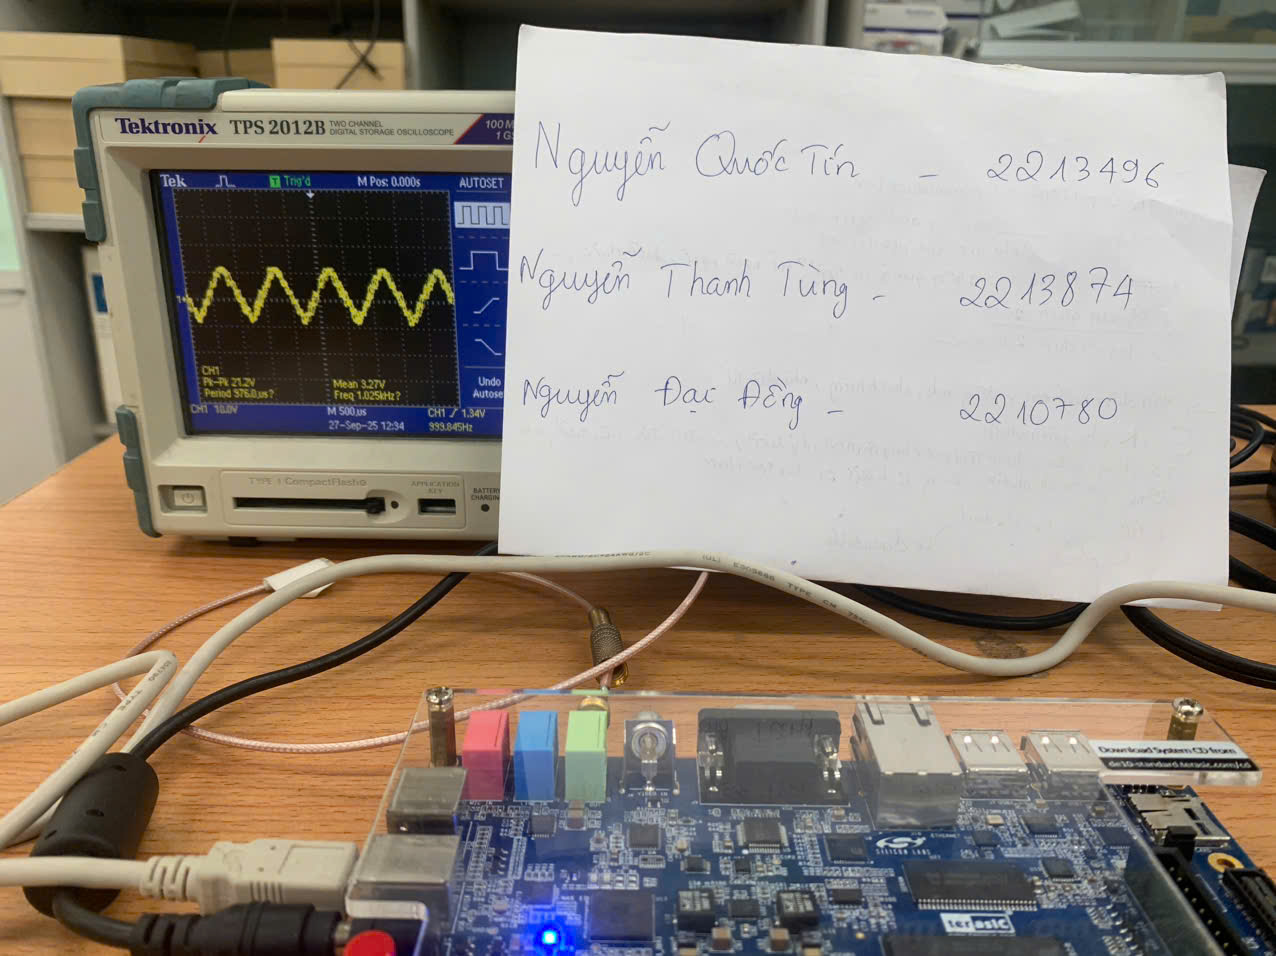
\includegraphics[width=.9\linewidth]{./my-chapters/my-images/Gen_wave/hinh5.jpg}
	\caption{Triangle waveform on Oscilloscope.}
\end{figure}

\begin{figure}[H]
	\centering
	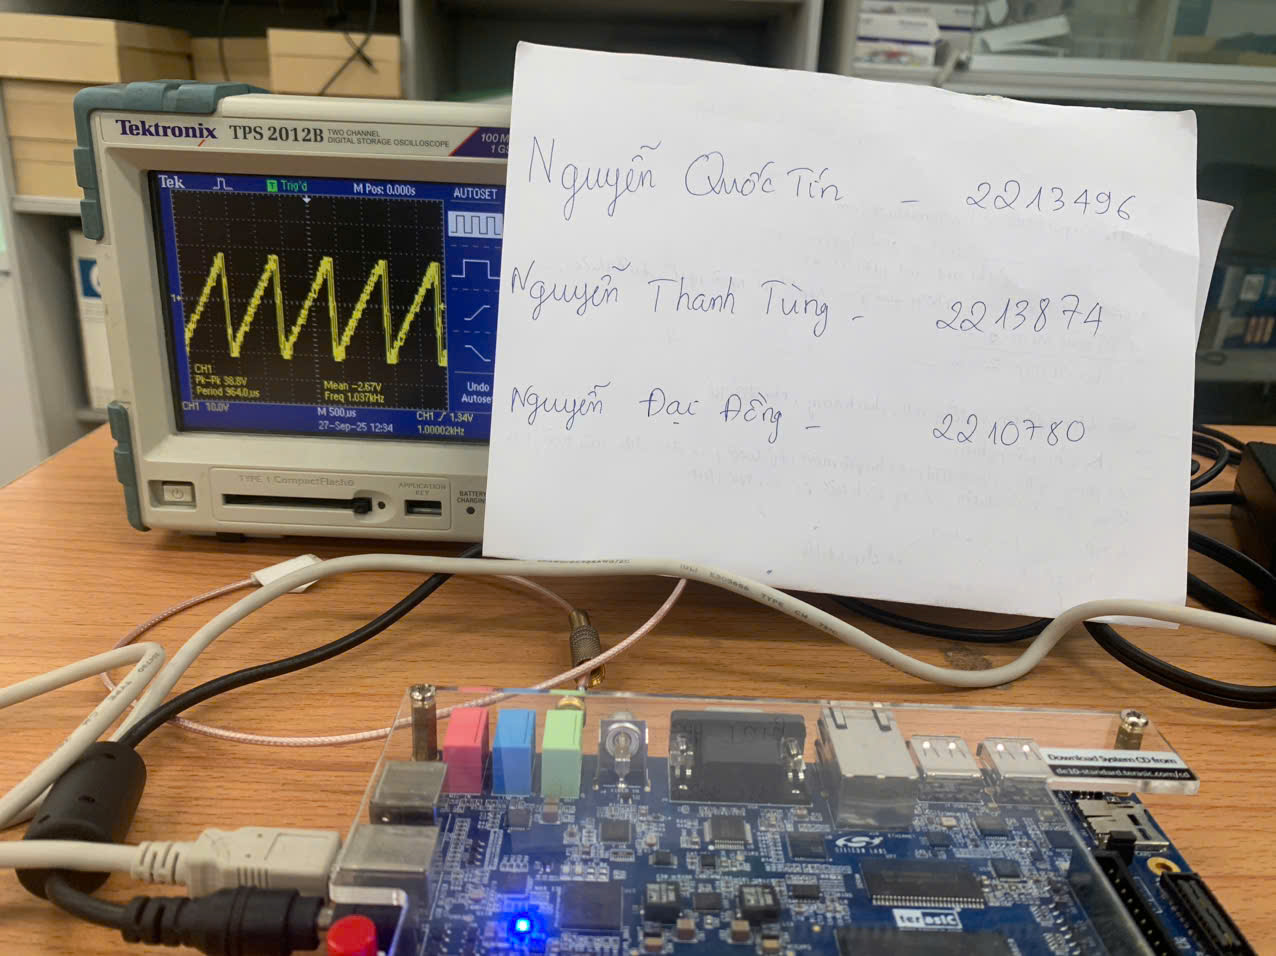
\includegraphics[width=.9\linewidth]{./my-chapters/my-images/Gen_wave/hinh4.jpg}
	\caption{Sawtooth waveform on Oscilloscope.}
\end{figure}

\begin{figure}[H]
	\centering
	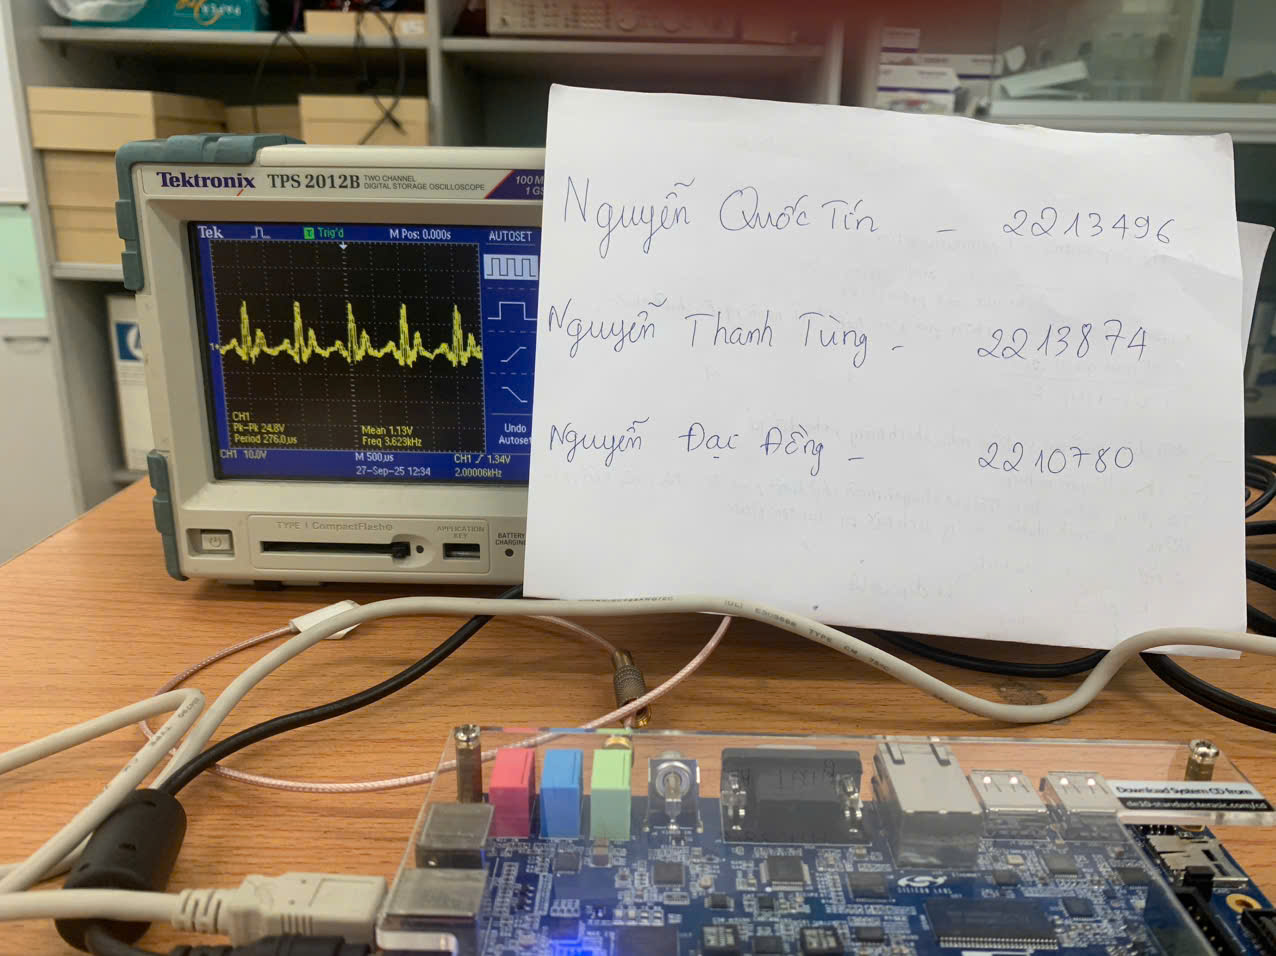
\includegraphics[width=.9\linewidth]{./my-chapters/my-images/Gen_wave/hinh3.jpg}
	\caption{ECG waveform on Oscilloscope.}
\end{figure}